% !TEX root = ../main.tex
\subsubsection{Offline Reconstruction} \label{sssec::offlinereconstruction}
    CLAS12 reconstruction and analysis relies on a data-stream processing framework called CLARA.
    CLARA provides a service-oriented architecture in which to build software applications composed of micro-services, linked together by data-stream pipes.
    The service-oriented framework allows for each engine to be encapsulated, helping guarantee a long lifetime and code modularity \cite{gyurgyan2016}.

    A service receives input data, processes it, and produces output data, where the I/O is organised into tabular structures called ``banks'' whose structure is configured by the specific service developer.
    A service reacts to an input data stream, processes it, and passes processed data to the next service in the data-flow path.
    As a result, the CLAS12 data processing application is versatile and flexible, since the application building blocks can be improved individually and replaced with no need for structural changes in the framework.
    % The CLAS12 services are extensions of an abstract reconstruction engine, which includes common components such as initialisation and event processing methods.
    % This approach reduces and simplifies the development of an individual micro-service and enforces a common structure.

    Data reader services access the detector decoded data stored in banks.
    Each entry for the decoded detector hits is a row in a bank.
    A row includes detector element identifiers (sector, layer, component, and order), and digitised detector data, such as signal charge, amplitude, time, or pedestal, depending on the specific system.
    Similar bank structures are created at the decoding stage for the various quantities needed for event reconstruction, such as hits, clusters, tracks, etc.
    The services that implement the reconstruction algorithms pertaining to the CLAS12 subsystems fill these banks, which are subsequently appended and written out to a file by a data-persistence service.

    The services running the reconstruction algorithms access the various banks as input and produce output banks needed for the subsequent algorithms in the reconstruction chain.
    The order in which the services are chained reflects the overall CLAS12 event reconstruction sequence and subsystem dependencies.
    First, charged particle tracks are reconstructed in both the Central and Forward Detector tracking systems based on the position of the recorded hits in the different detectors (i.e. using strip positions or wire locations).
    This procedure is referred to as ``hit-based'' tracking.

    In parallel, hits recorded in the other detectors are processed to reconstruct the energy and time of the associated particle interaction.
    These are matched to the reconstructed tracks by the Event Builder (EB) service, based on hit
    position and time information.
    Unmatched hits are retained as neutral particle candidates.
    At this stage, the EB can reconstruct the event ``start time'', or the time of the interaction between the beam and target, and identify the reconstructed particles.
    Once the event start time is determined, a second iteration of forward tracking can be performed to implement the so-called ``time-based'' tracking, which also incorporates the drift times in the Drift Chambers \cite{ziegler2020}.

    An overview of the reconstruction application service composition detailing these dependencies is shown in Figure \ref{fig::recon_chain}.

    \begin{figure}[t]
        \centering\frame{
        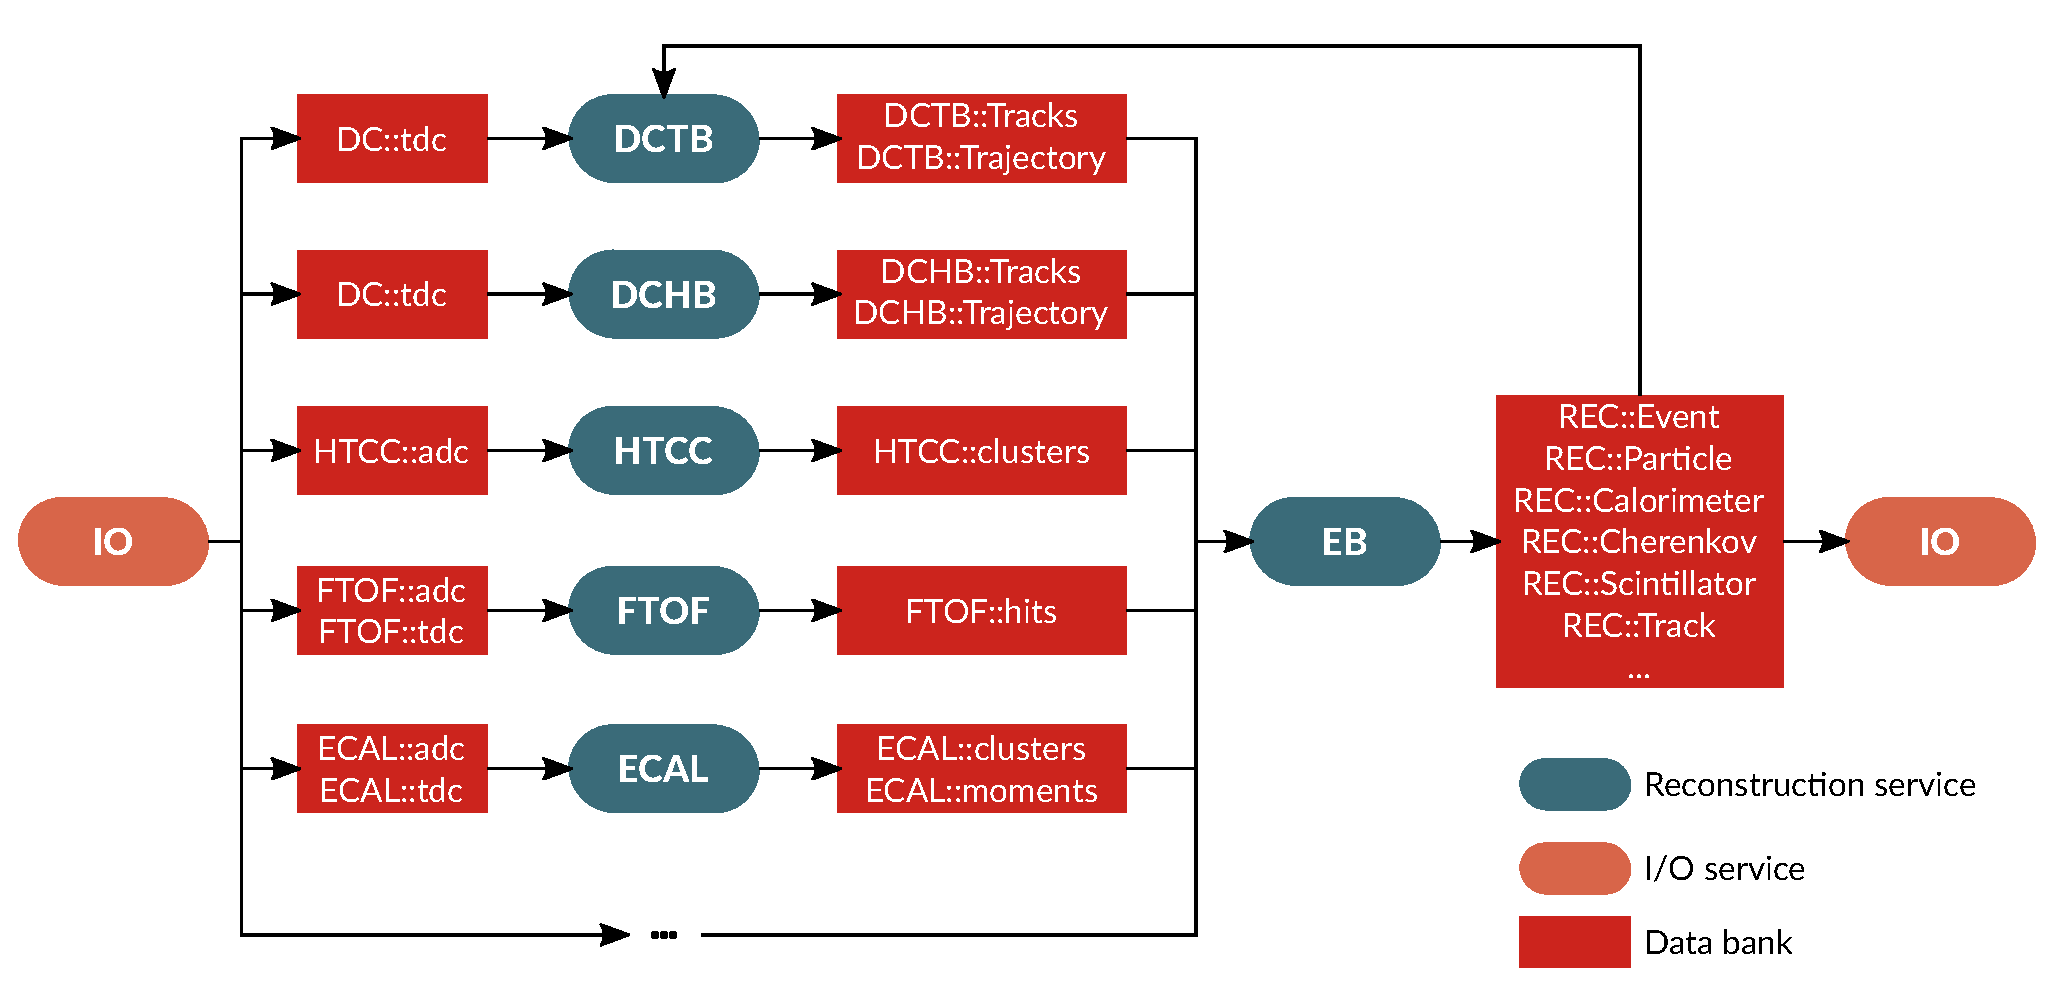
\includegraphics[width=\textwidth]{11experiment/img/23recon_chain.pdf}}
        \caption[CLAS12 Reconstruction Chain.]{Graphical representation of the CLAS12 interdependencies between services and banks.
        The I/O service reads events from the input file and distributes them to the reconstruction services chain for processing.
        Each service reads the relevant banks, applies the reconstruction algorithm, and provides output banks that are passed to the next service in the chain.
        The Event Builder (EB) service is executed as last in the chain; it collects the relevant banks from all CLAS12 subsystems services and produces event, particle, and detector response banks that are written to the output file.}
        \label{fig::recon_chain}
    \end{figure}

\paragraph{Tracking}
% --+ Introduction +------------------------------------------------------------
    Charged particle tracking is the key element of the CLAS12 event reconstruction.
    It is separated into the reconstruction of tracks in the central tracker system and the forward tracking system.

    In the forward region, the torus magnet bends charged particles inward toward the beamline or outward of it depending on their charge.
    At full nominal current, the $\int Bdl$ varies from $2 \text{Tm}$ at $5\degree$ to $0.5 \text{Tm}$ at $40\degree$.
    The forward tracking system in charge of tracking in this region is comprised of the Forward MicroMegas Tracker (FMT) and the Drift Chambers (DC).

    In the central region, the $5 \text{T}$ solenoidal magnetic field bends charged tracks into helices.
    In it, the central tracking system is comprised of the Silicon Vertex Tracker (SVT) and the Barrel MicroMegas Tracker (BMT), which together form the Central Vertex Tracker (CVT).

% --+ Reconstruction +----------------------------------------------------------
    \begin{wrapfigure}{l}{0.50\textwidth}
        \centering\frame{
        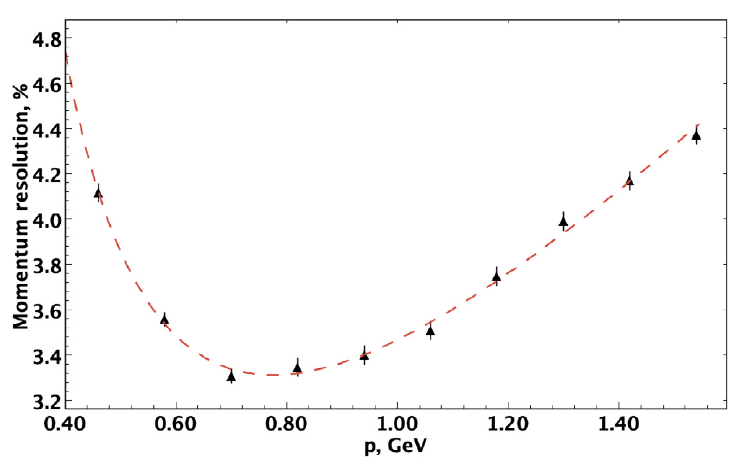
\includegraphics[width=\linewidth]{11experiment/img/23cvt_pres.png}}
        \caption[CVT momentum resolution vs. momentum.]{Momentum resolution vs. momentum of simulated protons in the CVT without background.}
        \label{fig::cvt_pres}
    \end{wrapfigure}

    For both systems, track reconstruction comprises algorithms for pattern recognition and track fitting. Hit objects, corresponding to the passage of a particle through a particular detector component, require the transformation of an electronic signal into a location of the track’s
    position in the detector subsystem geometry.
    A hit is defined as a detector element represented by a geometric object, for example, a line representing a strip in the central tracker.
    These objects then form the input to the pattern recognition algorithms.

    \begin{figure}[t]
        \centering\frame{
        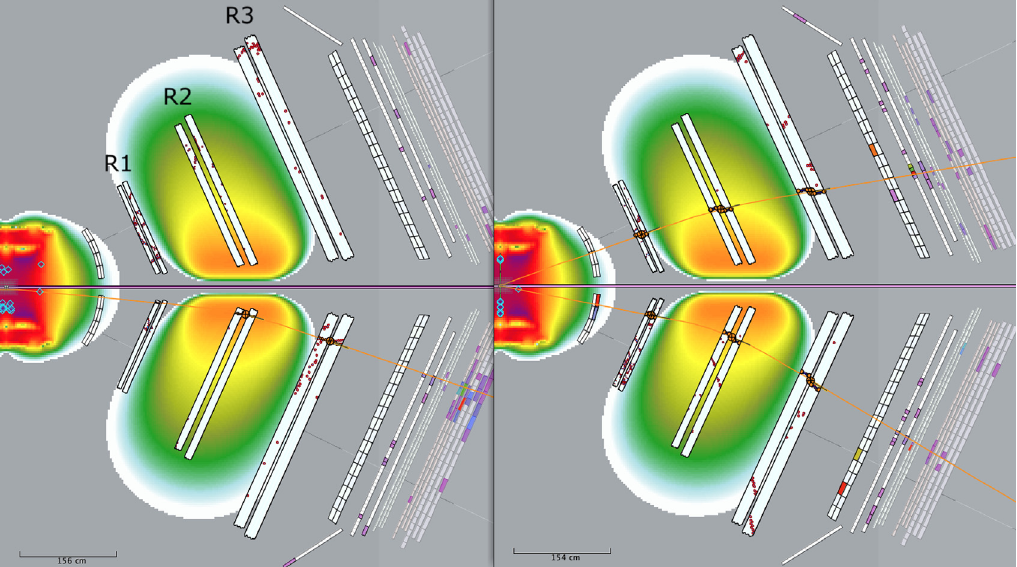
\includegraphics[width=\textwidth]{11experiment/img/23ced_event.png}}
        \caption[Particle going through DC.]{Views from CLAS12 Event Display (ced) of charged particle tracks in the DC showing cut-views to highlight different pairs of sectors of the CLAS12 Forward Detector.
        The coloured detector elements are the registered hits and the orange lines are the result of track reconstruction using the hits in the DC.
        The coloured areas about the detectors represent the regions of magnetic field from the torus and the solenoid.
        In these views the beam is incident from the left and the target is located in the middle of the solenoid (at the left edge of the image).}
        \label{fig::ced_event}
    \end{figure}

    Pattern recognition involves the identification of clusters of hits and the determination of the spatial coordinates and corresponding uncertainties for the hits and clusters.
    At the pattern recognition stage, hits that are consistent with belonging to a trajectory (such as a particle track) are identified.
    This set of hits is then fit to the expected trajectory with their uncertainties, incorporating the knowledge of the detector material and the detailed magnetic field map.
    An illustration of a particle going through the DC can be seen in Figure \ref{fig::ced_event}.

% --+ Performance +-------------------------------------------------------------
    The momentum resolutions in the central and forward trackers as a function of momentum are shown in Figures \ref{fig::cvt_pres} and \ref{fig::dc_pres} respectively.
    The distributions are fit with a function of the form $\sqrt{a + bx^2 + c/(1 + d/x^2)}$.
    In both distributions, the worsening of the resolution at low momentum is due to multiple scattering effects.
    The resolution also worsens as a function of momentum after a minimum is reached due to poorer track curvature resolution.

    \begin{wrapfigure}{r}{0.50\textwidth}
        \centering\frame{
        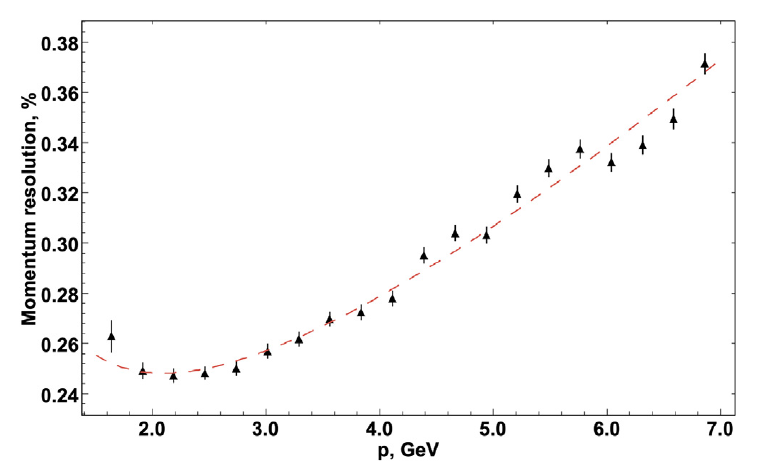
\includegraphics[width=\linewidth]{11experiment/img/23dc_pres.png}}
        \caption[DC momentum resolution vs momentum.]{Momentum resolution vs. momentum in the DC evaluated using pions simulated at $\theta = 15\degree \pm 5\degree$ and at $\phi = 0 \pm 5\degree$ without background.}
        \label{fig::dc_pres}
    \end{wrapfigure}

    For central tracking, an average CVT reconstruction efficiency of $87.3\%$ is obtained from a simulated proton sample with momenta in the range from $0.5$ to $2.5 \text{GeV}$.
    A slight drop of efficiency is observed for tracks with momenta less than $600 \text{MeV}$.
    The higher curvature of small $\text{p}_\perp$ tracks results in an increase in inefficiency due to acceptance effects.
    The dominant source of inefficiency is the gaps between the sensitive volumes for the BMT and the SVT.

    For forward tracking, the momentum resolution in the DC is evaluated using tracks simulated at $\theta = 15\degree \pm 5\degree$ and at $\phi = 0 \pm 5\degree$.
    This is to ensure that most tracks are within the sensitive volume.
    Furthermore, the DC momentum resolution is correlated with the polar angle since the track curvature is determined from the magnetic field intensity, which is higher at lower angles in the torus field.
    These resolutions are obtained from a Monte Carlo sample that does not include out-of-time backgrounds or misalignments of the tracking volumes \cite{ziegler2020}.

\paragraph{Particle Identification}
% --+ Introduction +------------------------------------------------------------
    The Particle Identification (PID) numbering scheme presented here was introduced by the Particle Data Group (PDG) in 1988 \cite{yost1988}.
    It is intended to aid in interfacing between the various generators, simulators, and analysis packages used in particle physics.
    The system was then revised and adapted in 1998 to allow the systematic inclusion of undiscovered and hypothetical particles \cite{particle1998}.
    The system used in this thesis comes from the most recent version as of the writing of this document, cited from the 2020 Review of Particle Physics by the PDG \cite{particle2020review}.

    The Event Builder (EB) is a service in the reconstruction chain, and performs a series of functions:
    It collects information from the upstream services; correlates information from the sub-detectors into particles; performs a general particle identification scheme; and organises the resulting information into a standardised, persistent data bank structure.
    The service is run twice with identical algorithms, once using hit-based tracks, and later with time-based tracks.
    As mentioned before, the results of the hit-based EB are used to initialise time-based tracking.

% --+ Forming particles +-------------------------------------------------------
    In defining a reconstructed charged particle in CLAS12, the EB assumes that an assignment will be made for each reconstructed track in both the FD and the CD.
    The associated calorimeter, scintillator, and Cherenkov detector responses are then assigned to that particle based on geometric coincidences between the detector responses and the track, with matching criteria corresponding to the resolution of a given detector.
    The geometric matching is based on the DOCA between the track and the response.
    A similar procedure is followed for creating neutral particles, except the seeding is presently with unassociated ECAL for the FD and CND for the CD responses instead of tracks.

% --+ Event start time +--------------------------------------------------------
    A start time is assigned to the entire event and serves as the most precise reference time on which all time-based particle identification relies.
    This is based on the optimal charged particle candidate in the FD with an associated FTOF timing response.
    The EB assigns the start time based on the highest energy electron in the ECAL.
    If there is no electron in the ECAL, it next looks for a positron in the ECAL.
    If there is no lepton, the next track in the priority list is a forward-going positive track (assumed to be a $\pi+$).
    Finally, if there is no forward-going positive track, it looks for a forward-going negative
    track (assumed to be a $\pi-$).
    When looking for $\pi+$ or $\pi-$ tracks, only the candidate with the highest momentum in each group is considered.

    A parallel event start time is determined from the FT to facilitate physics analyses and triggers where the primary scattered electron is at very forward angles in the FT.
    In this case, all combinations of charged particles in the FT and the FD are considered.
    The particle in the FT is assumed to be an electron, whereas all hadron mass hypotheses are considered for the FD tracks.
    The combination with the best time coincidence is chosen.
    The timing of the resulting FT electron is then used to assign the start time.
    A correction to the start time is then performed using the RF signal from the accelerator, combined with the reconstructed event vertex position.
    This effectively aligns the event start time to the best measure of the beam-bunch arrival time at the target.
    The uncorrected, measured vertex time of a particle, $t_v$, can be written as
    \begin{equation*}
        t_v = t - \frac{P_L}{\beta c},
    \end{equation*}
    where $t$ is the measured time response (e.g. in a scintillator), $P_L$ is the path length between the primary interaction vertex and that response, and $\beta c$ is the speed of the particle.
    We can then construct a correction to align this time with the closest beam bunch time at the target, using
    \begin{align*}
        \Delta t_{RF} &= t_v + \frac{z_0 - z_v}{c} - t_{RF} - \frac{N}{2f_{FR}}, \\
        \Delta t^\prime_{RF} &= \text{mod}(\Delta t_{RF}, 1/f_{RF}) - \frac{1}{2f_{RF}},
    \end{align*} % TODO. Not all variables are explained? Try to see what they are from reconstruction.
    where $f_{RF}$ is the frequency of the accelerator, either $249.5 \text{MHz}$ or $499 \text{MHz}$, corresponding to $2.004 \text{ns}$ or $4.008 \text{ns}$ bunch spacings, $t_{RF}$ is the measured, calibrated RF time for the event, and $z_0$ is the target center and enters due to its use as a position calibration reference.
    The resulting RF- and vertex-corrected start time for the event is then given as
    \begin{equation*}
        t' = t_v - \Delta t^\prime_{RF}.
    \end{equation*}

% --+ Particle identification +-------------------------------------------------
    The next stage is a basic particle identification scheme.
    This is intended to be loose to accommodate a variety of physics analyses, while persisting the necessary information to easily tighten and improve the criteria later.
    For charged particles, first calorimetry and Cherenkov information is used to positively identify $e-/e+$ candidates in the FD.
    If the measured energy deposition is consistent with the expected sampling fraction of the ECAL, and the photoelectron response from the HTCC is consistent with $\beta \sim 1$, the particle is assigned as an $e-$ or $e+$ depending on sign of the curvature of the track from forward tracking with the DCs through the torus magnetic field.

    The remaining charged particles are then assumed to be hadrons and assigned an identity based solely on timing information, where the $p,K,\pi$ candidate giving the smallest time residual is assigned.
    This time residual is computed from the difference between the measured particle flight time and that computed for a given mass hypothesis.

    \begin{wrapfigure}{r}{0.49\textwidth}
        \centering\frame{
        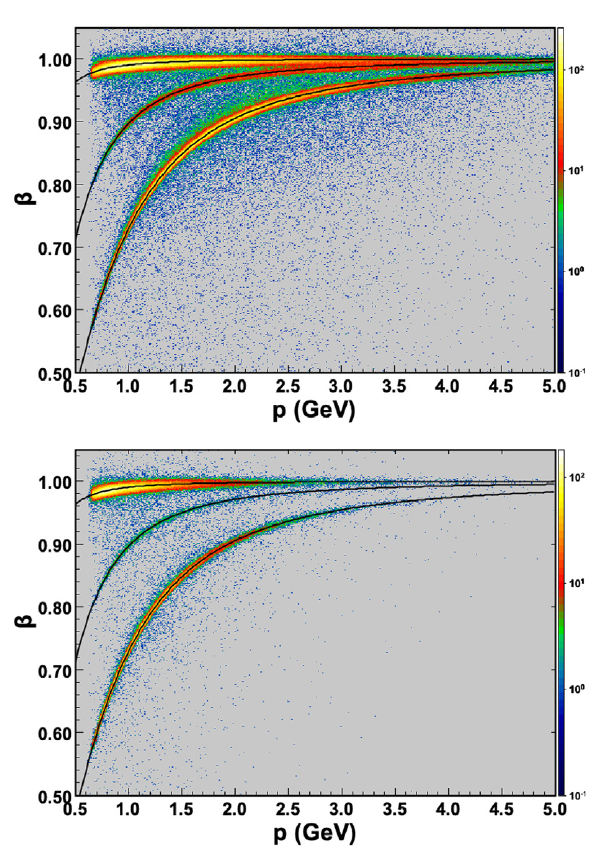
\includegraphics[width=\linewidth]{11experiment/img/23pos_pid.png}}
        \caption[Particle $\beta$ vs. momentum for positively charged tracks.]{Particle $\beta$ vs. momentum from simulation data for positively charged tracks with their start time from an electron in the FD (top plot) or in the FT (bottom plot).}
        \label{fig::pos_pid}
    \end{wrapfigure}

    Figure \ref{fig::pos_pid} shows reconstructed $\beta$ vs. momentum distributions from beam data for forward-going positively charged hadrons using information from the FTOF and DC subsystems, where the electron is reconstructed either in the FD (top) or in the FT (bottom).
    The computed curves for the different mass hypotheses are overlaid.

    Identification of neutral particles assumes only neutrons and photons, differentiated only by timing and topological information.
    For the FD this is based on the ECAL, while for the CD it is based on the CND, and their reconstructed cluster positions are used to compute the particle travel path from the event vertex, assuming a straight-line trajectory.
    If the resulting measured $\beta$ is close to $1$, the particle is assigned as a photon, otherwise it is assigned as a neutron.
    For photons in the FD, the momentum is determined from its deposited energy and ECAL sampling fraction \cite{asryan2020}. % TODO. READ UP ON THIS FOR ANALYSIS WORK.
    For neutrons, the momentum is assigned based on the measured $\beta$, assuming the neutron mass.
    Figure \ref{fig::n_gamma} shows an example of $\beta$ reconstructed for neutrals in the FD showing separation of photons and neutrons.

    \begin{wrapfigure}{r}{0.50\textwidth}
        \centering\frame{
        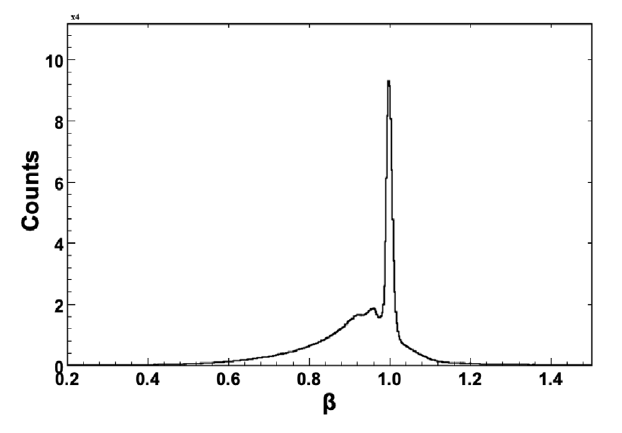
\includegraphics[width=\linewidth]{11experiment/img/23n_gamma.png}}
        \caption[$\beta$ distribution of neutrals.]{$\beta$ distribution for neutral particles as measured by the ECAL from simulation data, showing a sharp peak at $\beta = 1$ from photons and a broader, slower distribution from neutrons.
        }
        \label{fig::n_gamma}
    \end{wrapfigure}

% --+ Particle identification performance +-------------------------------------
    A particle identification quality factor in the form of a signed-$\chi^2$, or pull, is assigned based on the individual contributing detector subsystem responses and their resolutions.
    For $e-/e+$ identification the resolution-normalised distance from the expected ECAL sampling fraction is used, while for charged hadrons the resolution normalised time-difference is used.
    The resulting information is organised into standardised output bank structures for physics analysis.
    This includes the particle four-vectors, the associated detector responses, and global event information such as beam RF and helicity information.

    The accuracy of the particle identification algorithm that is currently implemented can be estimated from Monte Carlo simulations where the assigned particle identification can be compared to the true one.
    Table \ref{tab::rpid} shows the particle identification matrix for the FD (left) and CD (right).
    The values are based on simulations of electron-hadron or electron-photon pairs with hadron and photon momenta in the range from $1$ to $2.5 \text{GeV}$ and electron momenta in the range from $1$ to $9 \text{GeV}$.
    The diagonal elements correspond to the cases where the particle is correctly identified and the off-diagonal elements to the cases where the particle is misidentified ~\cite{ziegler2020}.
    % Another measure of the particle identification performance for neutrals is given by the reconstruction of $\pi^0$ decays to two photons.

    \begin{table}
        \caption{Particle identification matrix for the FD (left matrix) and CD (right matrix).
        The FD matrix is based on simulated hadrons and photons with momentum between $1$ and $2.5~\text{GeV}$, and electrons up to $9~\text{GeV}$.
        The CD matrix is based on simulated hadrons with momentum between $0.3$ and $1.1~\text{GeV}$.
        The diagonal elements are correctly identified, while the off-diagonal elements are misidentified.
        Detector inefficiencies are included.}

        \begin{tabularx}{\textwidth}{XXXXXXX|XXXXX}
            \hline
                     & \multicolumn{6}{l}{\textit{FD Truth}} & \multicolumn{5}{l}{\textit{CD Truth}}  \\
            \cline{2-12}
                     & $e$      & $\pi$ & $K$  & $p$  & $n$  & $\gamma$ &       & $\pi$    & $K$  & $p$  & $n$  \\
            \hline
            $e$      & 0.98     &       &      &      &      &          &       &          &      &      &      \\
            $\pi$    &          & 0.93  & 0.10 & 0.00 &      &          & $\pi$ & 0.84     & 0.14 & 0.00 &      \\
            $K$      &          & 0.03  & 0.80 & 0.00 &      &          & $K$   & 0.11     & 0.80 & 0.01 &      \\
            $p$      &          & 0.03  & 0.02 & 0.98 &      &          & $p$   & 0.03     & 0.04 & 0.95 &      \\
            $n$      &          &       &      &      & 0.66 & 0.01     & $n$   &          &      &      & 0.11 \\
            $\gamma$ &          &       &      &      & 0.14 & 0.95     &       &          &      &      &      \\
            \hline
        \end{tabularx}
        \label{tab::rpid}
    \end{table}
